\documentclass[a4paper]{article}
    
\usepackage[english]{babel}
\usepackage[utf8]{inputenc}
\usepackage{amsmath}
\usepackage{graphicx}
\usepackage{listings}
\usepackage{algorithm}
\usepackage{algpseudocode}
\usepackage{blindtext}
\usepackage[skins]{tcolorbox}
\usepackage[margin=1in]{geometry}
\lstset{
basicstyle=\small\ttfamily,
language=Java,
numbers=left,
stepnumber=1,
showstringspaces=false,
tabsize=1,
breaklines=true,
breakatwhitespace=false
}
\lstdefinestyle{nonumbers}
{numbers=none}

\graphicspath{ {images/} }
\title{CS3027 Continuous Assessment}

\author{Konrad Dryja}

\date{\today}

\begin{document}
\maketitle

\begin{abstract}
Results of my work throughout CS3027 Robotics during first semester 2017-2018 academic year.
\end{abstract}

\section{Preface}
\label{sec:Preliminaries}
\subsection{Preliminaries}

To be able to run all of nodes and packages, several adjustments to paths needs to be made, mainly path wise, so the exact components are visible to each other.
Let's start with the launch file located in launch\_files/assessment.launch \textendash{} it's going to be our starting point when running all the nodes written by me. Make sure to modify paths of map\_server, stage and add\_gaussian\_noise so they actually point to the actual location of the packages within your ROS environment. We will also have to modify our map files to utilise the provided files \textendash{} change \textquotedblleft{}image:\textquotedblright{} entry within launch\_files/map.yaml to reflect location of your map.png.
I have also made use of several extra pip packages which were tremendous help with dealing with concepts such as Gaussian Probability or array manipulations. Make sure that you have them installed and ready:
\begin{itemize}
    \setlength\itemsep{0.1em}
    \item Scipy (tested on version 1.0.0 / 25)
    \item Numpy (tested on version 1.13.3)
\end{itemize}
If not, be sure to install them using pip. If operating with multiple Python versions, make sure to use the correct version (i.e. pip2 / pip2.7 if using environment with main Python3). 
Environment used for development:
\begin{itemize}
    \setlength\itemsep{0.1em}
    \item Arch Linux / Ubuntu 16.04
    \item ROS Kinetic
    \item Python 2.7.14
    \item GCC 7.2.0
\end{itemize}

\subsection{Modifications to the provided files}
\label{sec:modifications}

It important to mention that I have slightly adjusted map.world file to slightly slow down simulation speed (from 50ms to 100ms) to match real time which ultimately avoids odometry readings discrepancies.
I have also altered launch file by removing dummy\_localization (as it is no longer needed and has been completely replaced by my own nodes) and appending real\_robot\_pose with rviz\_info which are uniform to use with every developed component.

\subsection{Project Overview}
\label{sec:overview}

Project consists of two ROS packages and one external file:
\begin{itemize}
    \setlength\itemsep{0.1em}
    \item assessment \textendash{} contains majority of the code produced for the purposes of CS3027.
    \item add\_gaussian\_noice \textendash{} provided by the course coordinator containing laser scan adjusted by random noise.
    \item pixeldraw.py (located in assessment/resources) \textendash{} pre-processing script to divide provided map onto cells which are used in path planning (see pathplanning.py module for further explanation).
\end{itemize}
And finally, beforementioned assessment package contains following files (later referred as nodes) \textendash{} all located in the scripts folder:
\begin{itemize}
    \setlength\itemsep{0.1em}
    \item real\_robot\_pose.py
    \item rviz\_info.py
    \item pathplanning.py
    \item drive.py
    \item localization.py
    \item image\_processing.py
\end{itemize}

\section{Design Choices}
\subsection{Map representation}
To begin this paragraph I wanted to briefly go through the concepts and ideas behind path-planning algorithms which could be utilised in terms of the course. Throughout my research on actual map representation I had looked into various methods such as:
\begin{itemize}
    \setlength\itemsep{0.1em}
    \item Occupancy grid
    \item Exact cell decomposition
    \item Approximate cell decomposition
    \item Potential field model
\end{itemize}
Ultimately I have settled for the approximate cell decomposition. One of the biggest turning points for me was the ease of implementation through a simple recursive call on 4 different areas which later could be easily converted to say a map, or graph representation of obtained cells. Due to the performance issues, speed and fact that I only have to perform decomposition only once (since I can assume that the map won't change) I have decided to do it only once and afterwards import the results into my actual ROS node through pickle python library (by compressing the created Graph structure after decomposition).
\begin{figure}[H]
    \centering
    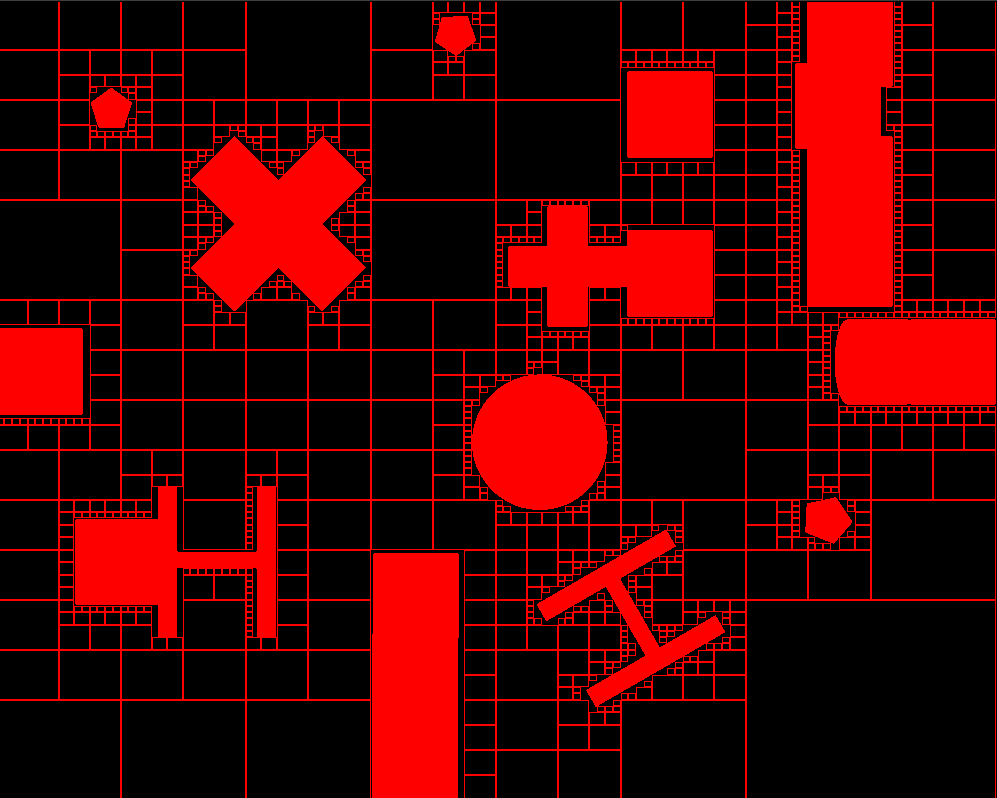
\includegraphics[scale=0.105]{img1}
    \caption{Representation of decomposed cells}
\end{figure}
Figure 1 represents how the map looks like post-decomposition. Every cell represents area where the robot can move freely without any collisions or issues. \textquotedblleft{}Robby\textquotedblright{} can also travel to any of the direct neighbouring cells as it wishes. Everything is based on the recursive call for which pseudo-code is included below:
\begin{algorithm}[H]
    \caption{Adaptive cell decomposition.}
    \begin{algorithmic}[1]
        \Procedure{Decompose}{$array, depth$}
            \If{no obstacle in $array$}
                \State \texttt{Mark $array$ as cell}
                \State \Return
            \Else
                \State{\Call{Decompose}{top left of $array$}}
                \State{\Call{Decompose}{top right of $array$}}
                \State{\Call{Decompose}{bottom left of $array$}}
                \State{\Call{Decompose}{bottom right of $array$}}
            \EndIf
        \EndProcedure
    \end{algorithmic}
\end{algorithm}
Nodes and files including logic for path-planning: pathplanning.py, resources/pixeldraw.py

\subsection{Pathplanning}
Now, I should receive approximately 500 discrete cells \textendash{} which is another advantage of the method over, say, occupancy grid where I would need to consider 1000*800 pixels \textendash{} those values quickly add up and it is important to reduce run-time as it may be crucial when the robot needs to act quickly.

I have utilised the graph and nodes structures that I used for the CS2521 continuous assessment which allows me to easily store each cell, its neighbours and distances to those neighbours. Afterwards implementing any of the path-planning algorithms becomes trivial since I only needed to code a simple A* using Euclidean distance as a heuristic function. All the operations are performed on the occupancy grid array (reshaped from 1d to 2d \textendash{} 800x1000) thanks to the implementation of functions allowing me to easily swap around Map Frame coordinates (e.g x=2.5, y=-3.5) to Occupancy Grid (e.g. row=253, column=575).

Last, but not least, to obtain the shortest path overall (given all goals) I had to implement a brute-force solution in non-deterministic polynomial time by getting every available permutations of those lists, getting shortest path out of all of those permutations and publishing the path to driving node.
\subsection{Driving}
As opposed to my friends who were focusing on proportional controllers and driving based on the distance remaining I have taken a slightly different stance which is driving based on the time elapsed. Pseudo-code below represents the through process and algorithm flow when running the node:
\begin{algorithm}[H]
    \caption{Driving module pseudo-code.}
    \begin{algorithmic}[1]
        \While{time elapsed * speed \textless{}= distance}
            \State keep moving forward\;
        \EndWhile
    \end{algorithmic}
\end{algorithm}
One of the issues that I have encountered is the fact that sometimes due to the computing inaccuracies the robot ends up slightly beyond the requested point. I believe it may be caused with the CPU overload and trying to catch up with ROS simulation. The problem probably could be avoided by instead of relying on time, I would base it on distance travelled \textendash{} both approaches have their drawbacks. Pseudo-code above is easily applied to the list of destinations that I have to visit obtained from path-planning module so the implementation becomes trivial. One thing to note is that due to my laptop's capabilities (where a VM performed even worse) I had to decide against using my own localisation solution to help the robot localise itself within the environment, instead I am utilising /base\_pose\_ground\_truth (while still having odom errors enabled which are corrected as-you-go).

\subsection{Localisation}
That is the part that I am the most proud of. I have managed to fully implement Monte Carlo Localisation as a node in my ROS project. It was probably the most difficult project and I had to consider plenty of approaches to the problem. The biggest issue wasn't choice of localisation method \textendash{} it was the actual act of perception and motion update that caused me the most problems, especially the former as it was exceptionally computational dependant constantly taking massive chunks of my CPU power.
\begin{figure}[H]
    \centering
    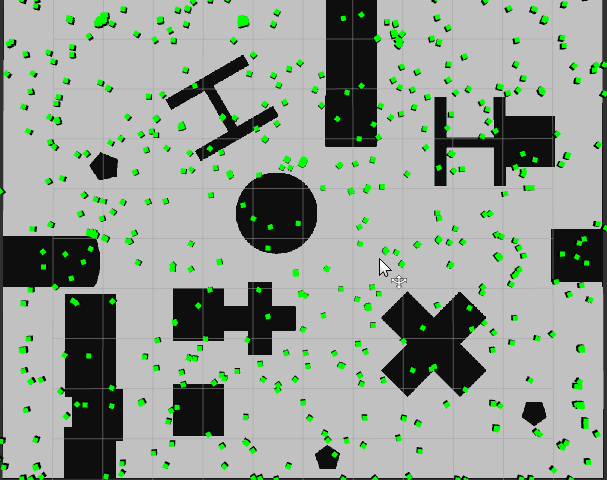
\includegraphics[scale=0.3]{img2}
    \caption{Particles as displayed in Rviz}
\end{figure}
To start off, I'm placing 800 random particles across the map (as shown on figure 2) \textendash{} each of them with three properties: X, Y and Theta. Now I needed a way to tell how likely it is for a particle to appear in a given position.

I have considered two methods of performing perception update at all \textendash{} use either Beam Sensor Model or Likelihood Field Model. Unfortunately I didn't quite comprehend the latter so I focused on the beam sensor model which in principle is trivial \textendash{} simply track every pixel that laser beam covers and check occupancy grid to see whether it is obstacle or not. If it is, return the expected distance \textendash{} and keep repeating till you reach the maximum distance which is 3 meters in our case. Once I have obtained my expected reading I referred to the actual \textendash{} obtained from the noisy scanner. Thanks to the access to the add\_gaussian\_noise I read out the properties such as standard deviation which I plugged into SciPy's Probability Density Function so I will get the proportional probability of how likely the reading is.

Now robot casts 30 different laser proximity beams. Due to the precious computation time I had to divide those by 6 leaving me with 5 of them \textendash{} which is more than enough in our environment. By adding all of those probabilities I got a total probability of given particle being at a given point of the map. So now I've got all my particles and their probabilities \textendash{} all is left is sampling. Simply pick 500 particles based on the weighted probability and add them to the next iterations. Remaining 300 are randomised again to allow recovery from errors.

As when it comes to clustering of the particles, the location obtained from my localisation is always based on the particle with the highest probability. Both the actual position and and believed position are printed to the console to check how accurate my reading are and for debugging purposes.

\subsection{Image processing}
Work in progress...



\end{document}